\section{Calibration}

This section presents the parameter estimation results and evaluates the model's ability to replicate observed trade and production patterns. Our estimation strategy follows the method of moments approach, targeting key structural relationships while ensuring computational stability through exponential parameter transformations.

\subsection{Parameter Calibration Strategy}

Our calibration follows a four-stage approach separating parameters by identification source. Each parameter group uses the most appropriate econometric method given the underlying economic structure. 

\subsubsection{Preference and Technology Parameters from Input-Output Data}

We extract structural parameters directly from the WIOD input-output tables following standard practices in the quantitative trade literature \citep{costinot2012TheReviewofEconomicStudies}. Expenditure shares are computed as:
\begin{align*}
\alpha_{nk} = \frac{\sum_i X_{nik}}{\sum_k \sum_i X_{nik}}
\end{align*}
where $X_{nik}$ represents country $n$'s total expenditure on sector $k$ products from all origins $i$, ensuring that $\sum_k \alpha_{nk} = 1$ for each country. Labor shares in production are calculated as:
\begin{align*}
\beta_{ik} = \frac{\text{Labor Compensation}_{ik}}{\text{Gross Output}_{ik}}
\end{align*}
Again, this satisfies the resource constraint $\beta_{ik} \in [0,1]$ Intermediate input coefficients are derived as sectoral input requirements:
\begin{align*}
\gamma_{ikk'} = \frac{\sum_j Z_{ijkk'}}{\sum_{l}\sum_j Z_{ijkl}}
\end{align*}
where purchases of sector $k'$ inputs by sector $k$ in country $i$ are normalized by gross output. These parameters satisfy the resource constraint $\sum_{k'} \gamma_{ikk'} = 1$ by construction. Tables \ref{tab:alpha} through \ref{tab:gamma_USA} in the appendix present the complete parameter matrices.

In the Appendix, we present the full set of estimated parameters derived from the WIOD data, including preference parameters $\alpha_{nk}$ (Table \ref{tab:alpha}), labor share parameters $\beta_{ik}$ (Table \ref{tab:beta}), and intermediate input coefficients $\gamma_{ikk'}$ (Tables \ref{tab:gamma_BRA} through \ref{tab:gamma_USA}). 

We can see some standard patterns, which we highlight below.

\paragraph{Preference Parameters} The expenditure shares (Table \ref{tab:alpha}) reveal expected consumption patterns. Services represent the largest expenditure category across all countries, consistent with the service economy dominance in modern economies. Developing countries (China, Brazil, India, Mexico) allocate higher expenditure shares to Food compared to developed economies, reflecting lower per capita incomes and Engel's law. Developed countries show higher relative spending on Construction, indicating greater infrastructure investment and housing consumption.

\paragraph{Labor Share Parameters} Labor shares (Table \ref{tab:beta}) display clear sectoral patterns. Service-oriented sectors (Services, Retail/Wholesale, Transport) exhibit high labor intensity, reflecting their people-intensive nature. Capital-intensive sectors (Energy, Manufacture, Metal) show low labor shares, consistent with their reliance on physical capital and technology. These patterns are consistent across countries, suggesting similar production technologies worldwide.

\paragraph{Intermediate Input Shares} The intermediate input matrices (Tables \ref{tab:gamma_BRA} through \ref{tab:gamma_USA}) display strong diagonal elements, indicating significant within-sector input usage. Services and Retail/Wholesale sectors serve as important input suppliers to most other sectors, reflecting their role as business services and distribution channels. These patterns remain consistent across countries, supporting the assumption of similar production technologies in our structural model.

\subsubsection{Trade Elasticity from Literature}

The trade elasticity $\theta$ is set to 6.53 following \cite{costinot2012TheReviewofEconomicStudies}, which represents the central estimate from their comprehensive analysis of bilateral trade patterns. This value lies within the consensus range of 2.84 and 12.86 established by the broader literature \citep{eaton2002Econometrica} and provides appropriate substitution elasticity for our multi-sector framework.

\subsubsection{Productivity Parameters via CDK Regression}

Productivity parameters $T_{ik}$ are estimated using the two-step procedure developed by \cite{costinot2012TheReviewofEconomicStudies}. We first run the reduced-form regression:
\begin{equation}
\log \pi_{nik} = \alpha_{ik} + \gamma_{nk} + \varepsilon_{nik}
\end{equation}
where $\pi_{nik}$ represents observed bilateral trade shares, $\alpha_{ik}$ are origin-sector fixed effects capturing comparative advantage, and $\gamma_{nk}$ are destination-sector fixed effects reflecting market access. Following CDK methodology, productivity parameters are recovered as:
\begin{equation}\hat{T}_{ik} = \exp\left(\frac{\hat{\alpha}_{ik}}{\theta}\right)
\end{equation}
This approach leverages the theoretical restriction that comparative advantage patterns in the model must match observed trade flows, providing robust identification of country-sector productivity levels. We also have some issues with multicollinearity in the regression, which we address by using matrix completion via low-rank matrix approximation with nuclear norm regularization \citep{mazumder2010spectral}. Table \ref{tab:technology} presents the estimated productivity matrix.

\subsubsection{Structural Estimation of Trade Costs}

The final stage estimates iceberg trade costs through structural method of moments, targeting exact replication of observed bilateral trade shares while satisfying general equilibrium constraints. We parameterize trade costs using an additive decomposition in log space:
\begin{equation}
\log d_{nik} = \log d_{ni} + \log d_{nk}^{\text{importer}} + \log d_{ik}^{\text{exporter}}
\end{equation}
where $d_{ni}$ captures bilateral geographic and institutional barriers, $d_{nk}^{\text{importer}}$ reflects destination-sector import barriers, and $d_{ik}^{\text{exporter}}$ represents origin-sector export facilitation. This decomposition reduces the parameter space from $N^2 \times K$ to $N(N-1) + 2NK$ while maintaining sufficient flexibility to match observed trade patterns. Without this our model would be underidentified given the limited number of observations.

We solve the method of moments system:
\begin{align*}
\min_{\boldsymbol{\theta}} &\quad \sum_{n,i,k} \left( \pi_{nik}^{\text{data}} - \pi_{nik}^{\text{model}}(\boldsymbol{\theta}) \right)^2 \\
\text{s.t.} & \quad \text{Trade Balance Constraint} \\
& \quad \text{Price Consistency Constraint}
\end{align*}
where $\boldsymbol{\theta}$ contains trade cost components $\{d_{ni}\}$, $\{d_{ik}^{\text{importer}}\}$, $\{d_{jk}^{\text{exporter}}\}$, along with wages $\{w_{ik}\}$ and prices $\{p_{ik}\}$ as endogenous variables. Table \ref{tab:trade_costs} presents the estimated trade cost components.

\subsection{Calibration Performance and Parameter Estimates}

\paragraph{Productivity Parameters} Productivity estimates (Table \ref{tab:technology}) confirm expected comparative advantage patterns. Developed countries (USA, EU, UK) exhibit high productivity in Services and Chemicals, reflecting their technological sophistication and human capital endowments. China demonstrates strong productivity in Textiles and Manufacture, consistent with its manufacturing specialization. Brazil shows high productivity in Food production, aligning with its agricultural comparative advantage. These patterns validate the CDK regression approach for identifying productivity differences.

\paragraph{Tariff Structure} Baseline tariff data (Tables \ref{tab:tariff_BRA} through \ref{tab:tariff_USA}) reveal expected patterns. Non-tradable sectors (Services, Retail/Wholesale, Transport) have zero tariffs by construction. USMCA members (USA, Canada, Mexico) maintain low bilateral tariffs, reflecting their trade agreement. Canada also has preferential access to UK and EU markets. China exhibits relatively high protection levels across sectors, while India maintains low tariffs with the UK, possibly reflecting historical trade ties.

\paragraph{Trade Cost Decomposition} Bilateral trade costs (Tables \ref{tab:bilateral_costs}, \ref{tab:exporter_effects}, \ref{tab:importer_effects}) show geographic proximity effects. Neighboring countries (USA-Canada-Mexico, EU-UK) have lower bilateral costs. Notable exceptions include high costs between India and China, suggesting significant institutional or logistical barriers. Labor mobility assumptions do not substantially affect these estimates, indicating that trade cost identification is separate from labor market adjustments.

The structural estimation achieves excellent fit to observed trade patterns ($R^2 = 0.9331$). Figure \ref{fig:trade_flows_fit} demonstrates strong correlation between predicted and observed bilateral trade shares across both mobile and immobile sectors, validating our decomposed trade cost specification. The model replicates key stylized facts: the gravity relationship between trade flows and economic size, the home bias in consumption patterns, and the sectoral variation in trade intensities. Moment matching performance indicates that our four-stage calibration strategy successfully identifies the structural parameters while maintaining computational efficiency.

\begin{figure}[H]
    \centering
    \begin{subfigure}{0.48\textwidth}
        \centering
        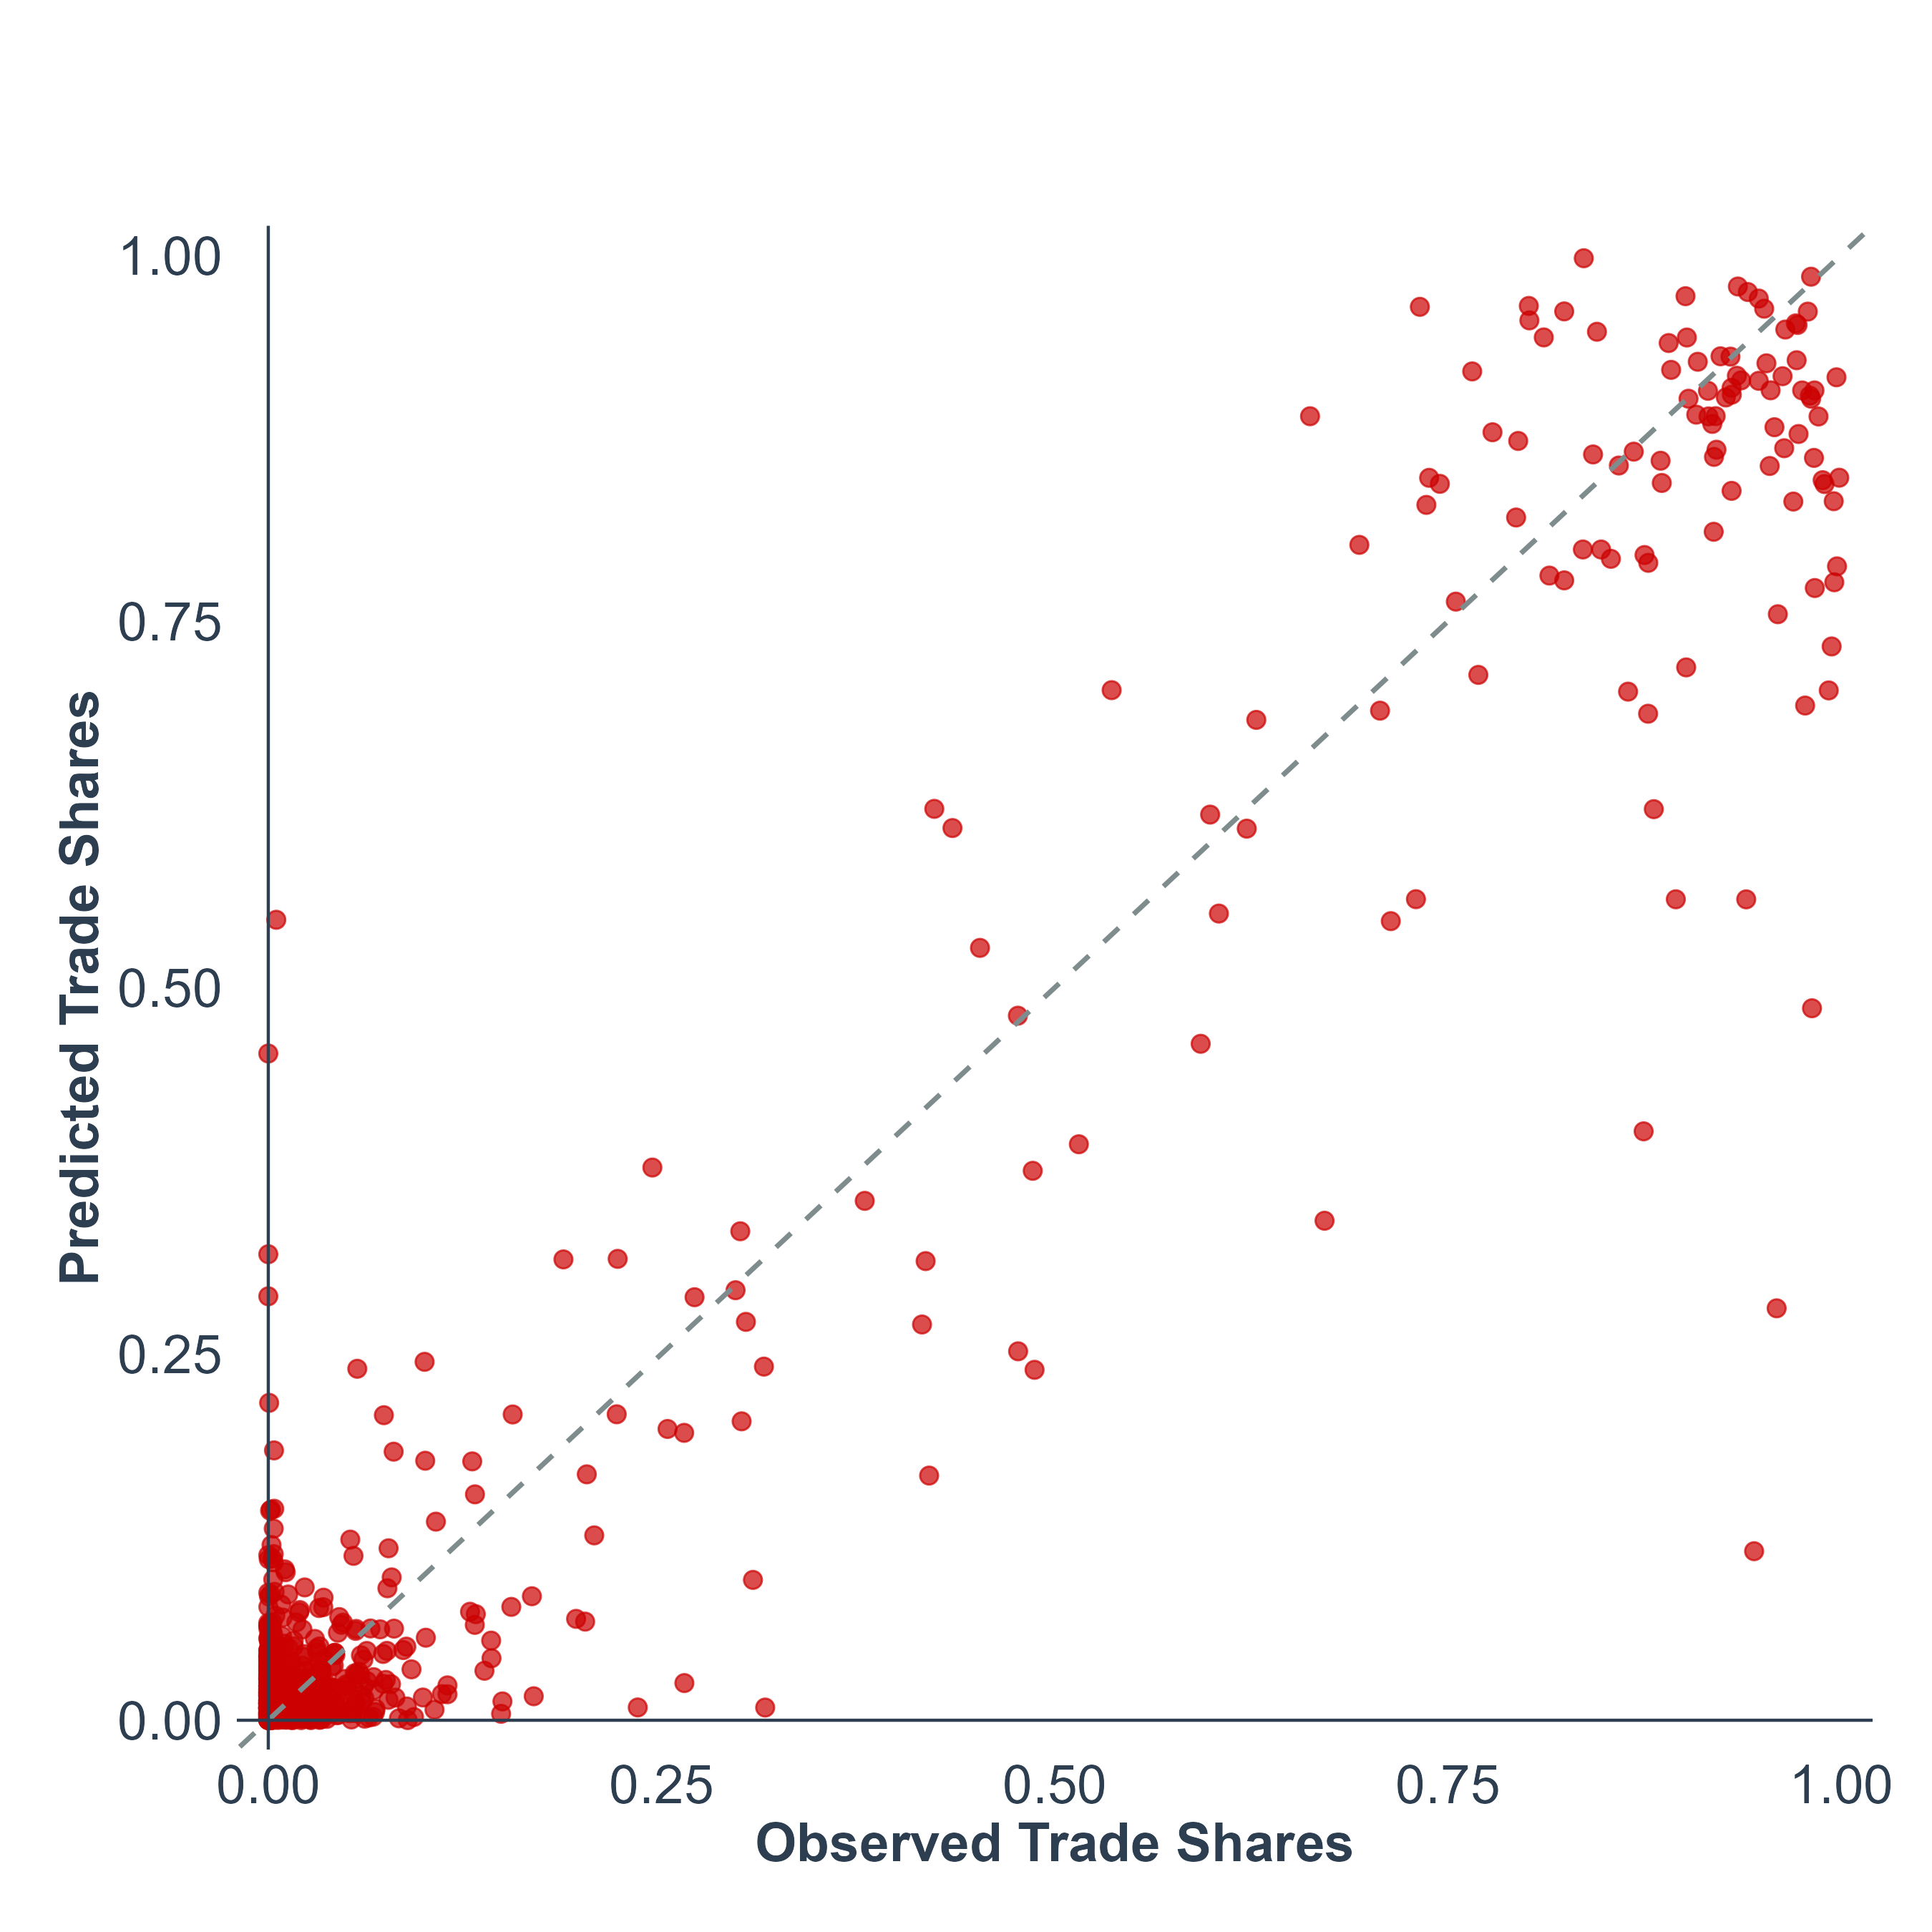
\includegraphics[width=\textwidth]{code/figures/trade_flows_fit_mobile.png}
        \caption{Mobile Sectors}
        \label{fig:trade_flows_fit_mobile}
    \end{subfigure}
    \hfill
    \begin{subfigure}{0.48\textwidth}
        \centering
        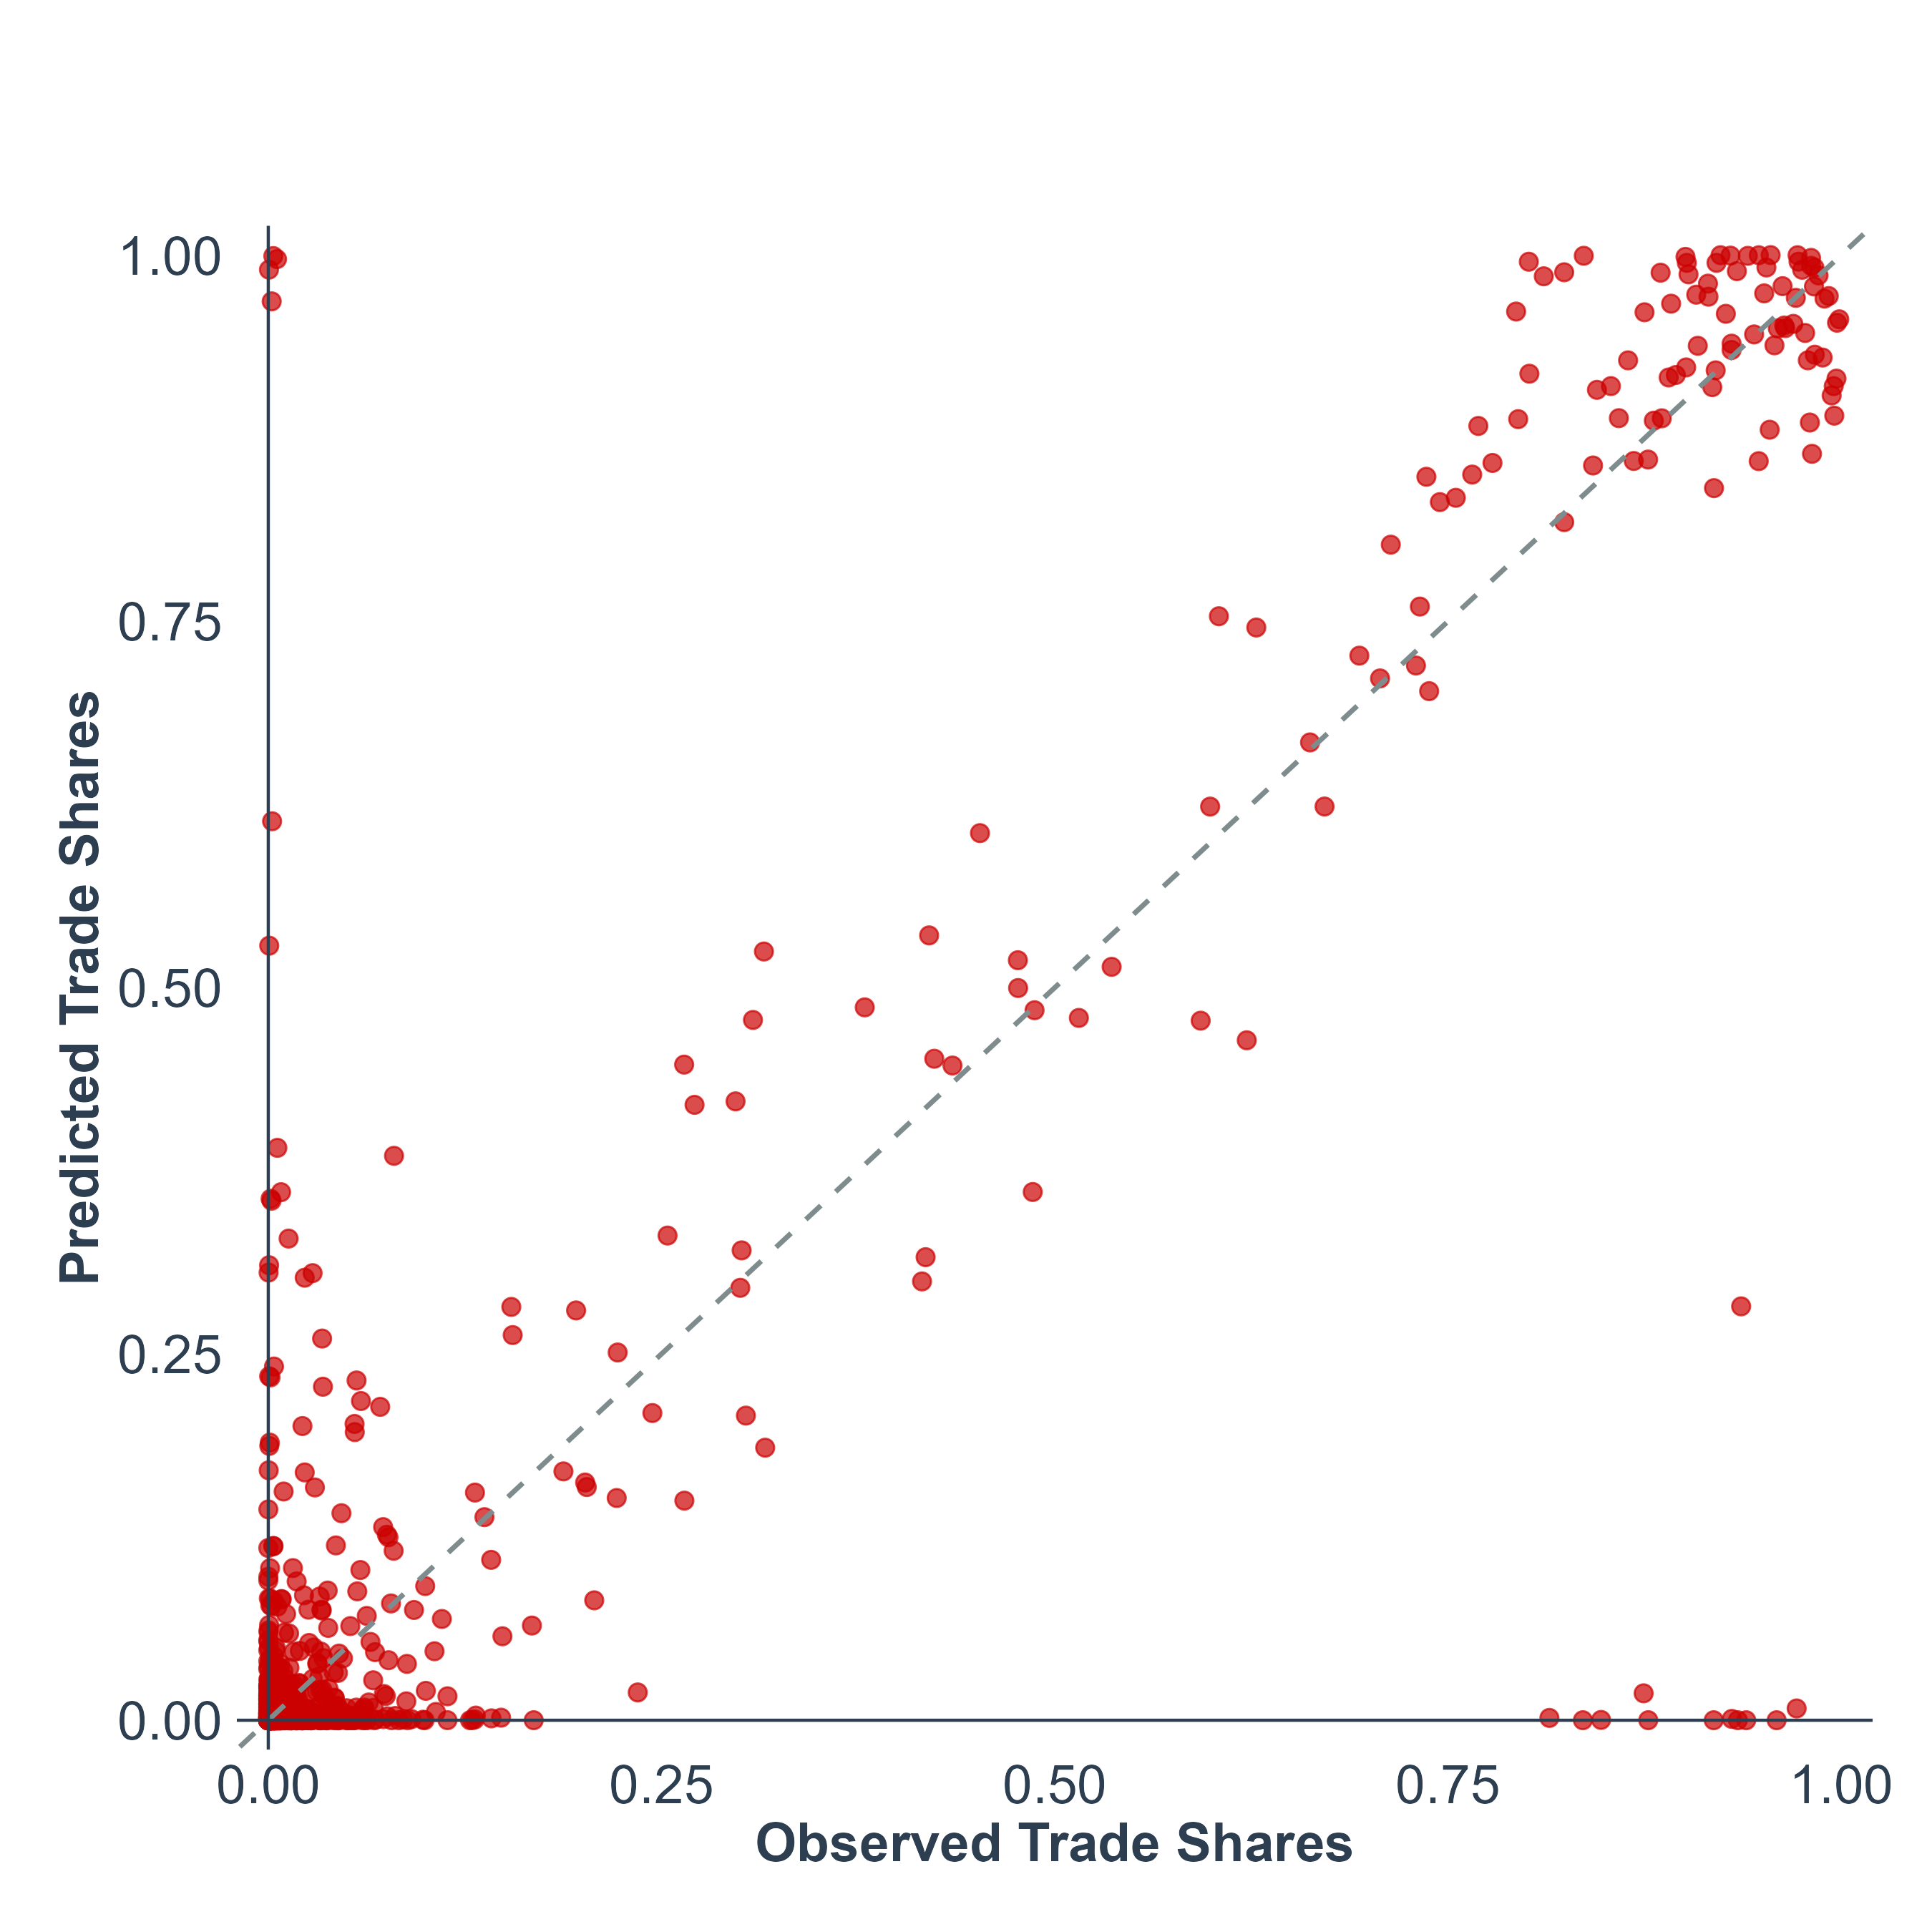
\includegraphics[width=\textwidth]{code/figures/trade_flows_fit_immobile.png}
        \caption{Immobile Sectors}
        \label{fig:trade_flows_fit_immobile}
    \end{subfigure}
    \caption{Model Fit: Predicted vs. Observed Bilateral Trade Shares}
    \label{fig:trade_flows_fit}
\end{figure}

However, when we look at GDP shares, the fit is very poor, as shown in Figure \ref{fig:gdp_fit}. This is likely due to the fact that we are not targeting GDP shares in our calibration, and the model is not flexible enough to match both trade shares and GDP shares simultaneously given the limited number of parameters. This suggests that future work could explore alternative parameterizations or additional data sources to improve the model's ability to replicate observed production patterns while maintaining trade flow accuracy.

\begin{figure}[H]
    \centering
    \begin{subfigure}{0.48\textwidth}
        \centering
        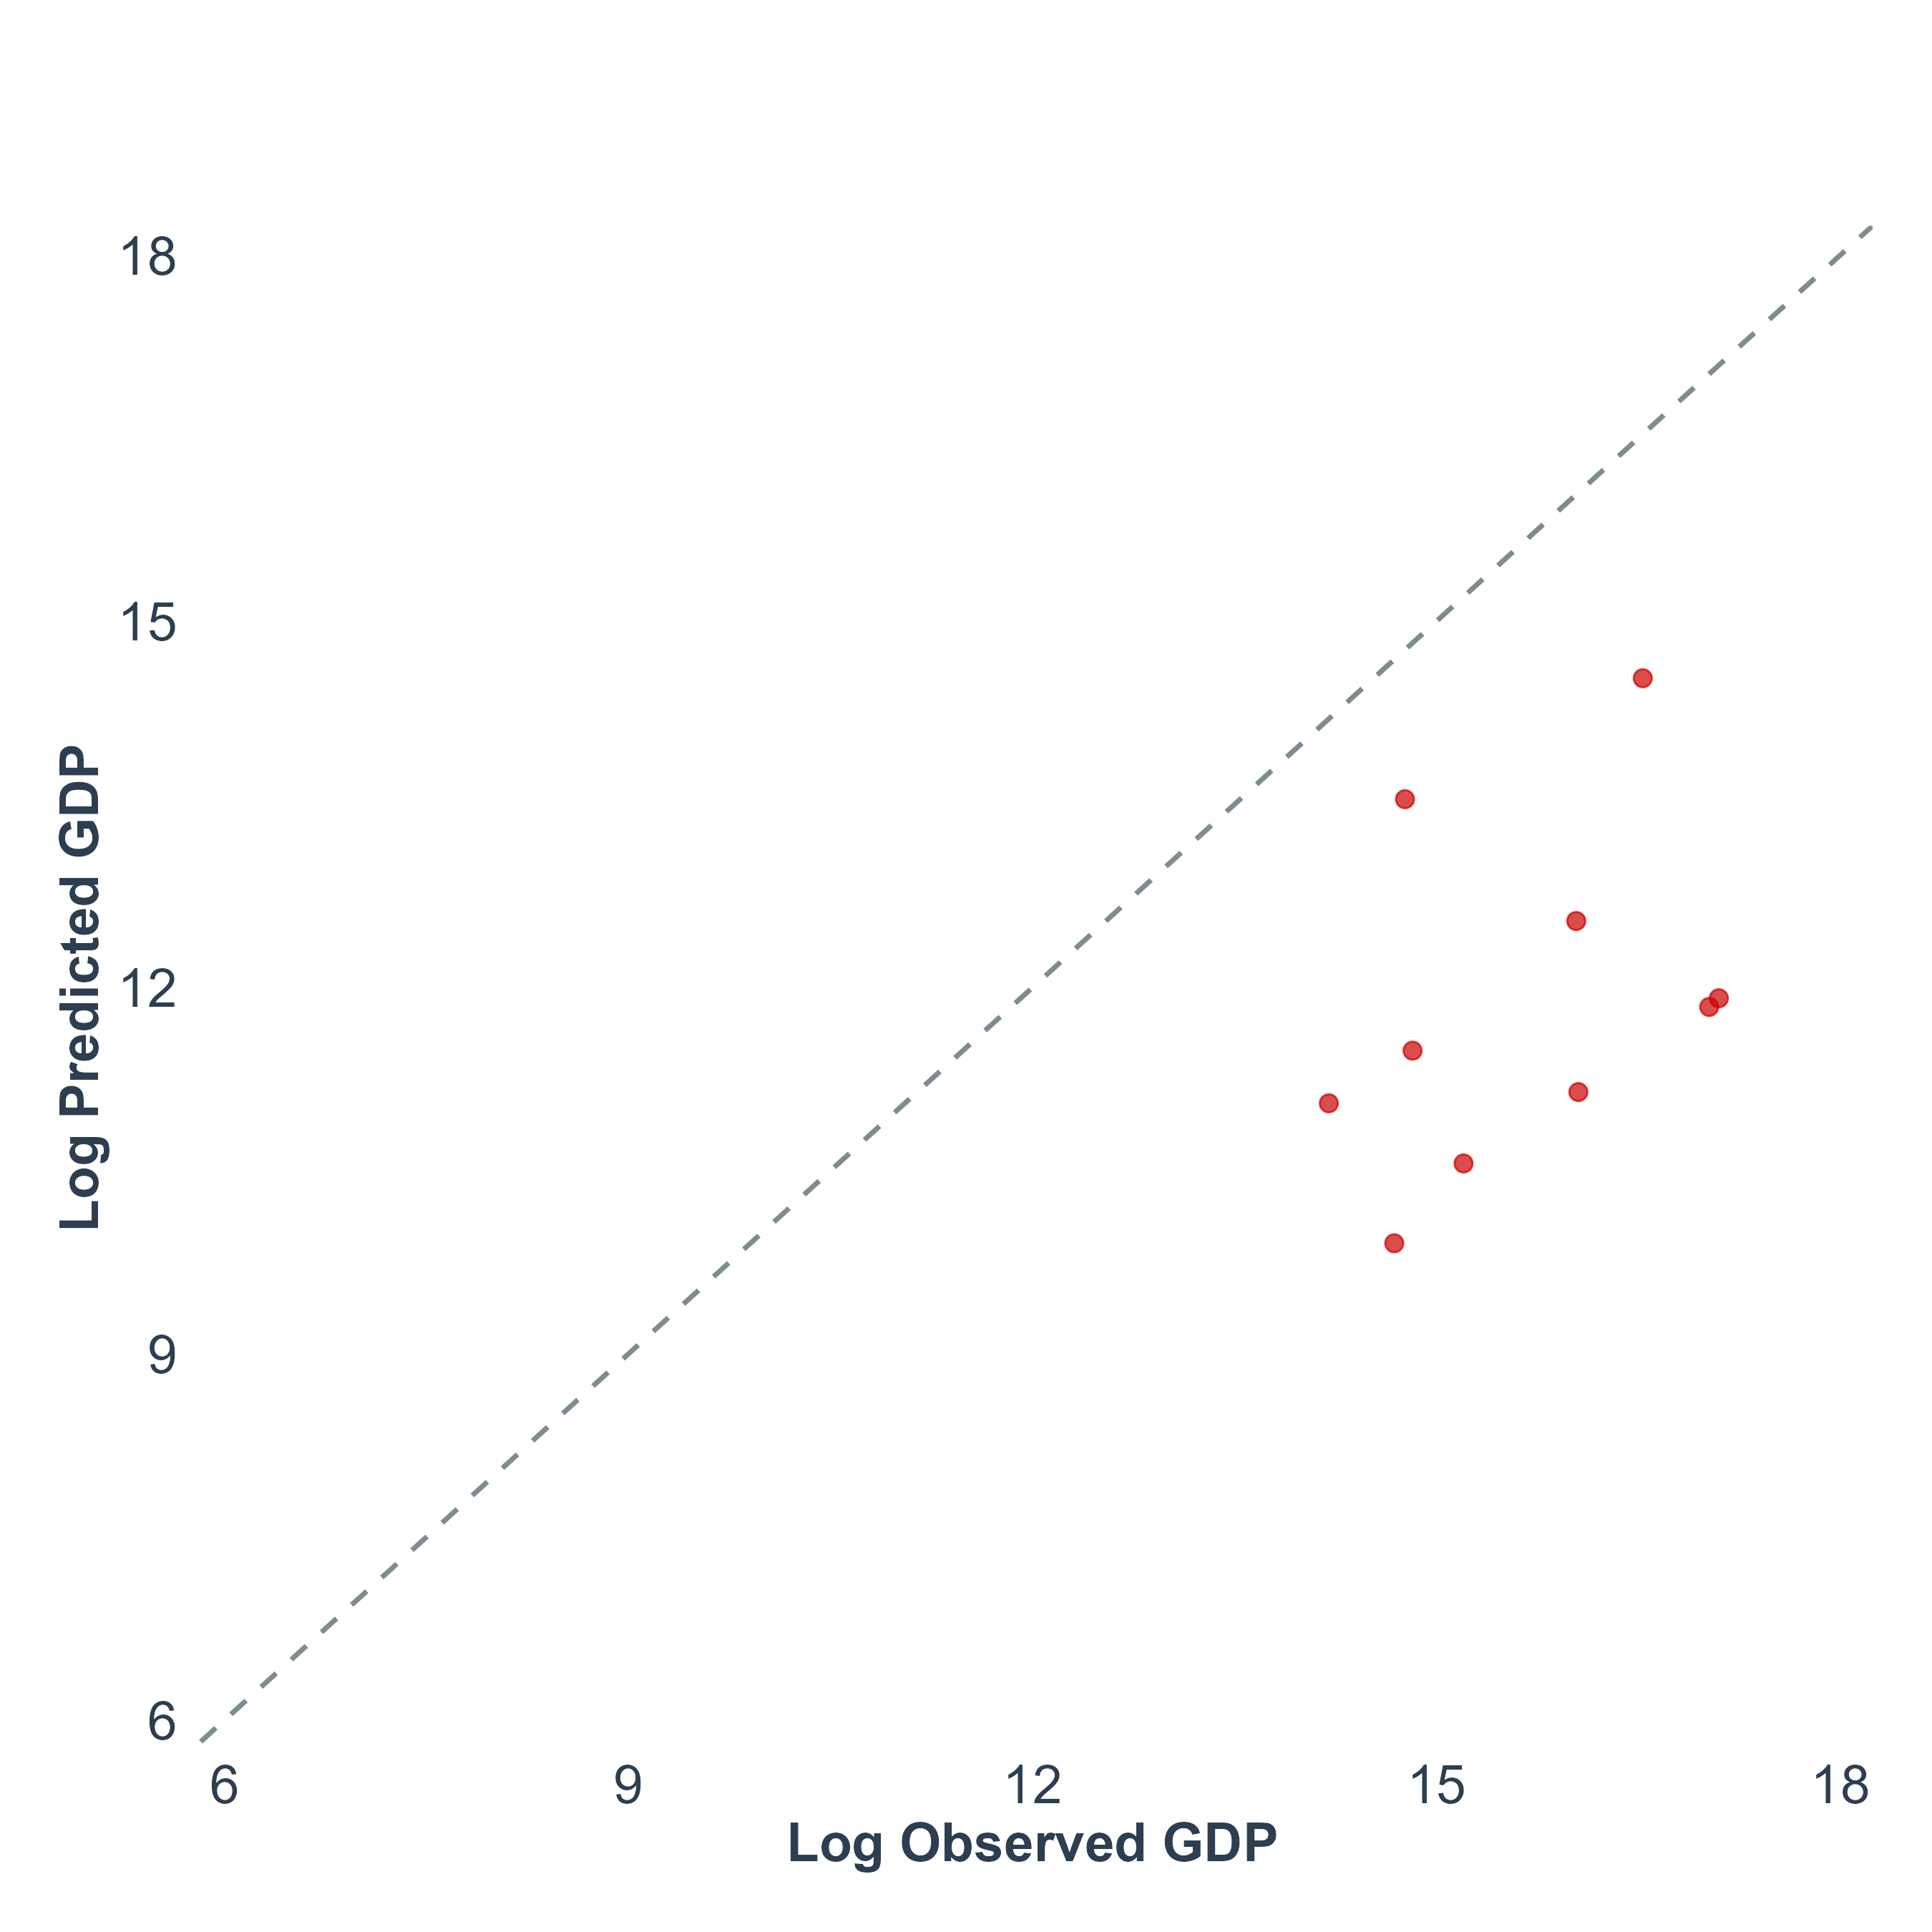
\includegraphics[width=\textwidth]{code/figures/gdp_fit_mobile.png}
        \caption{Mobile Sectors}
        \label{fig:gdp_fit_mobile}
    \end{subfigure}
    \hfill
    \begin{subfigure}{0.48\textwidth}
        \centering
        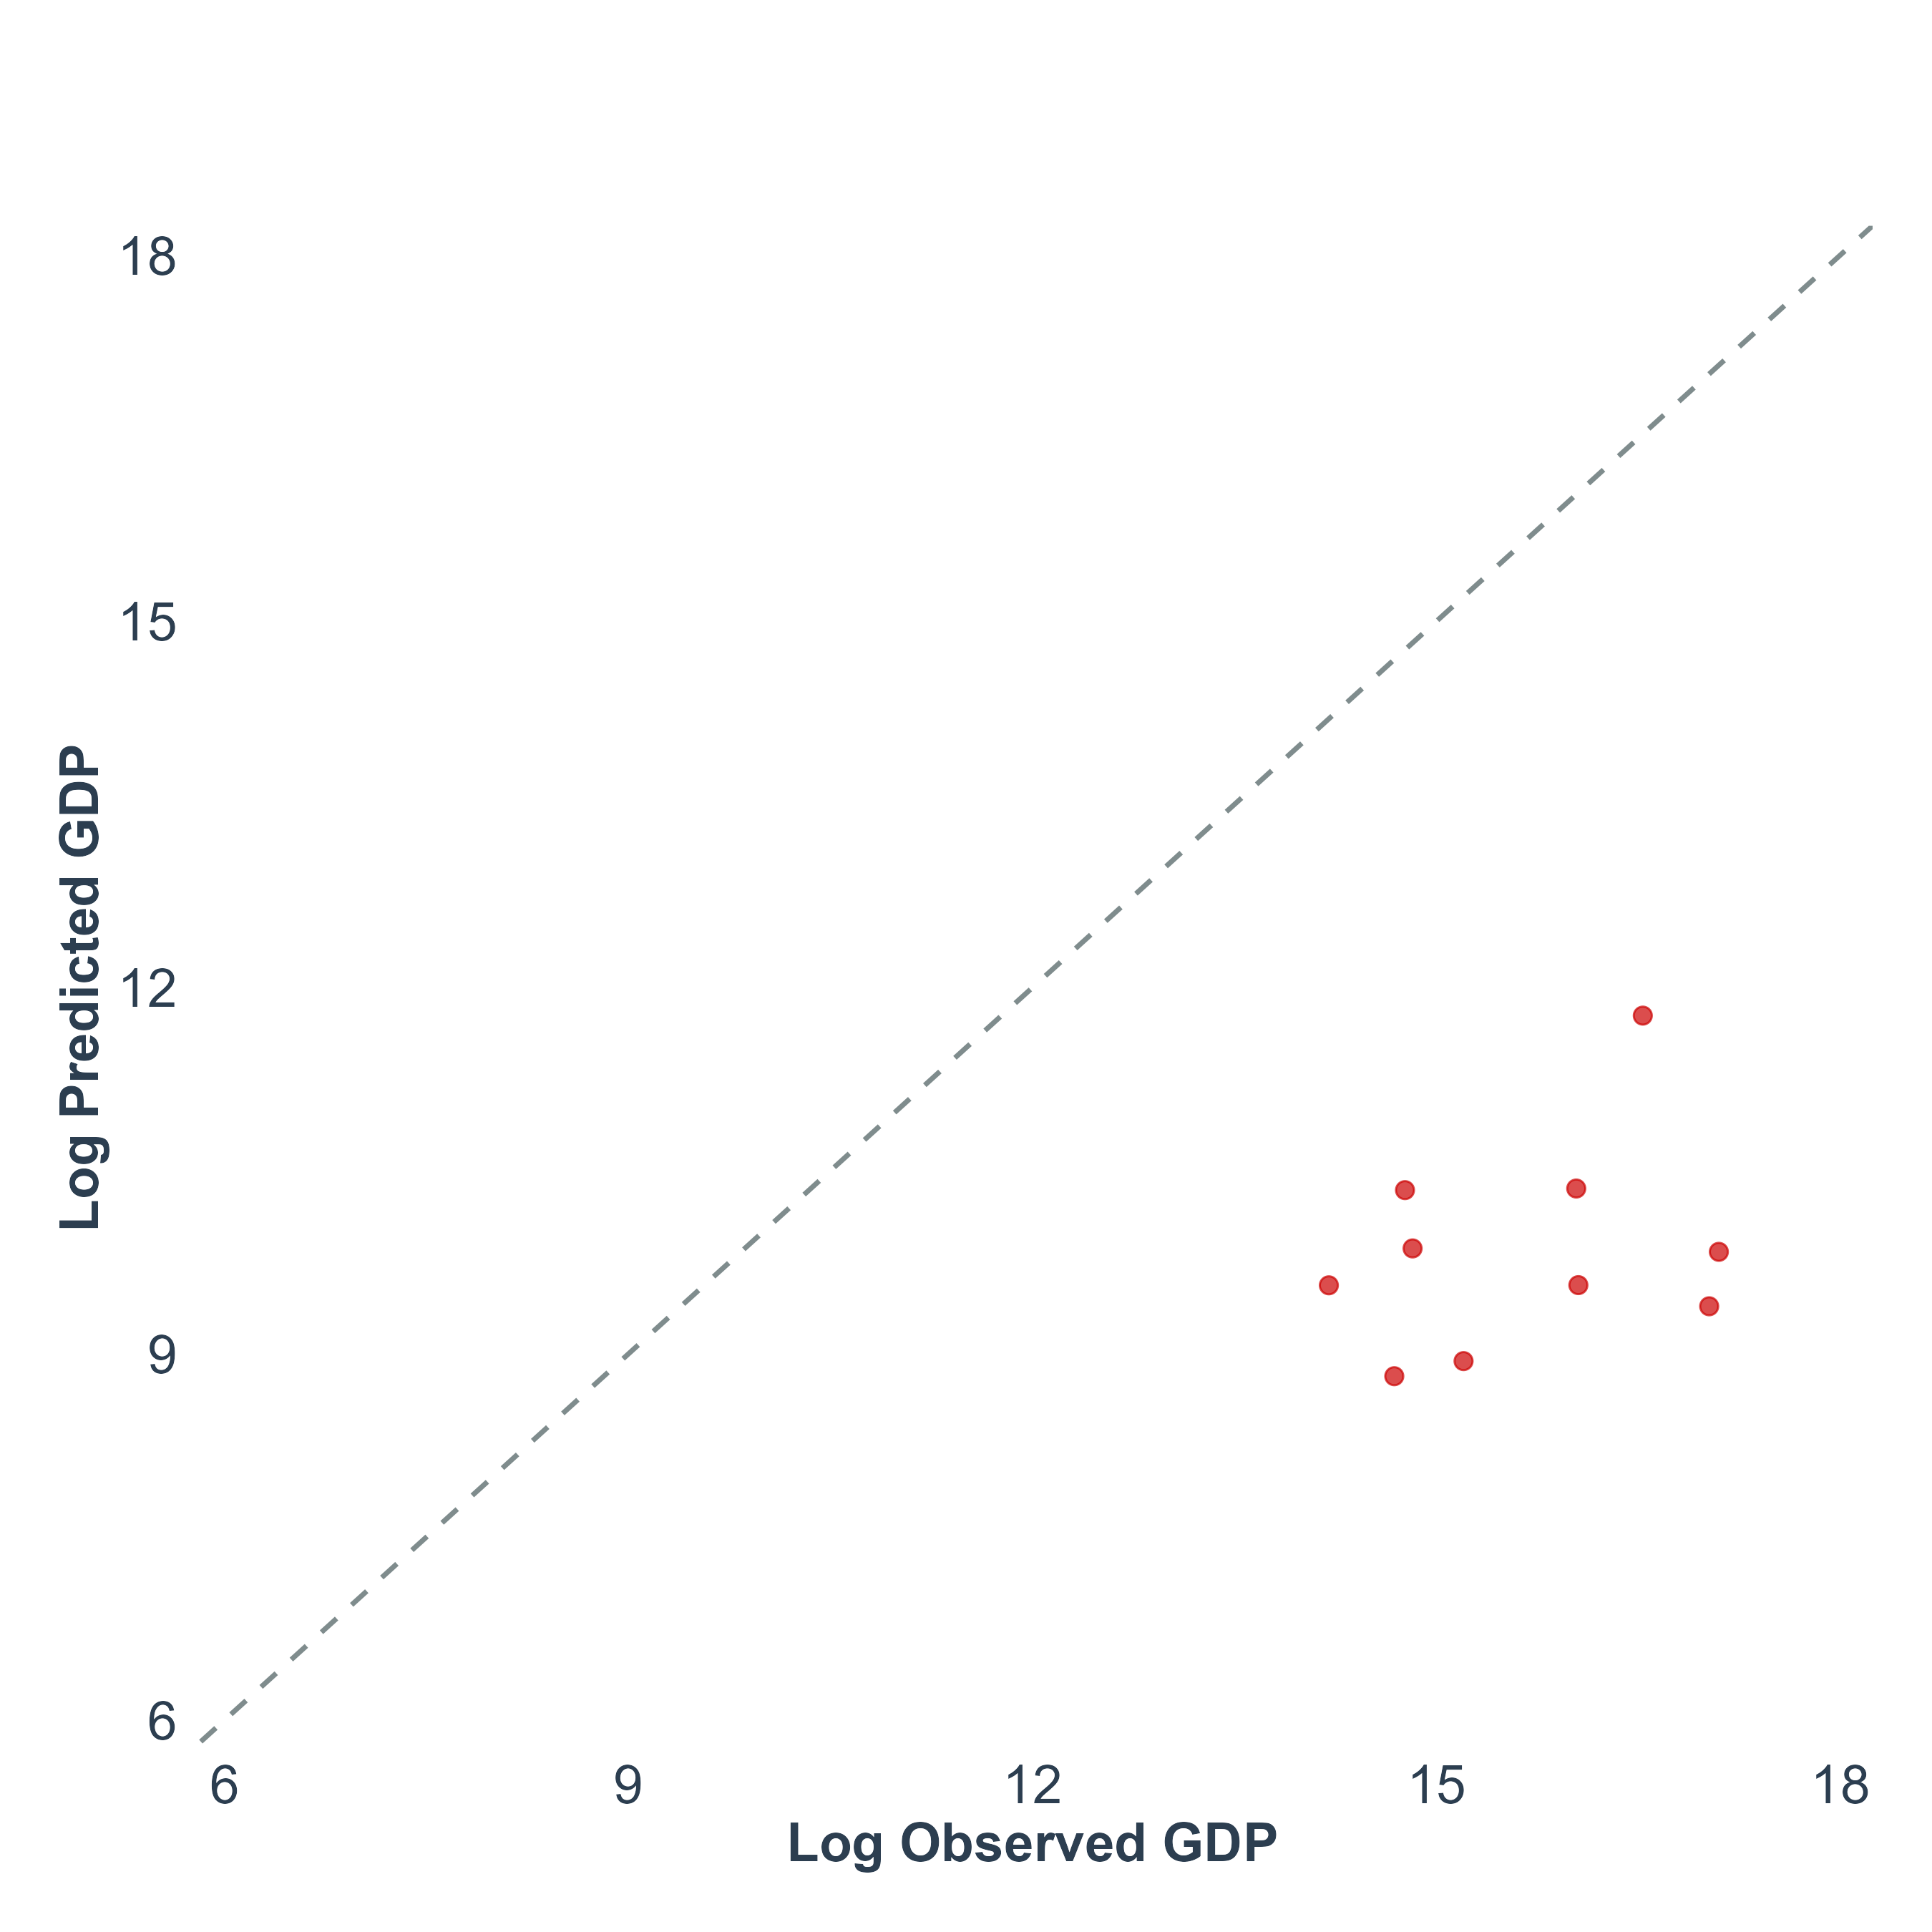
\includegraphics[width=\textwidth]{code/figures/gdp_fit_immobile.png}
        \caption{Immobile Sectors}
        \label{fig:gdp_fit_immobile}
    \end{subfigure}
    \caption{Model Fit: Predicted vs. Observed GDP Shares}
    \label{fig:gdp_fit}
\end{figure}


The calibrated model satisfies all equilibrium conditions within numerical tolerance. Trade balance is achieved: $\sum_{i,k} \pi_{ink} X_{ik} - \sum_{i,k} \pi_{nik} X_{nk} = 0$ for all countries, and price consistency relationships are verified: the sectoral price indices $p_{nk} = \left[\sum_{i} \left(\frac{c_{ik}(1+\tau_{nik})d_{nik}}{T_{ik}^{1/\theta}}\right)^{-\theta}\right]^{-1/\theta}$ match computed values. 